\documentclass[11pt]{article}

\usepackage[paper=a4paper,margin=0.75in]{geometry}
\usepackage{setspace}
\usepackage{amsmath,amsfonts,amssymb,amsthm}
\usepackage{graphicx}
\usepackage{hyperref}
\usepackage{mathrsfs}
\usepackage{bbm}
\usepackage[bottom]{footmisc}
{
	\newtheorem{assumption}{\textit{Assumption}}
	\newtheorem{definition}{\textit{Definition}}
	\newtheorem{theorem}{\textit{Theorem}}
}
\usepackage{fancyhdr}
\pagestyle{fancy}
\rhead{\today}
\lhead{Dynamic Multiple-Agent Discrete Choice}

\newcommand\blfootnote[1]{%
	\begingroup
	\renewcommand\thefootnote{}\footnote{#1}%
	\addtocounter{footnote}{-1}%
	\endgroup
}

\begin{document}
\onehalfspacing

\section{Dynamic Discrete Games: Theory to Estimation}

\blfootnote{These notes are based on Howard Smith's lectures from the 2018-2019 academic year.\\
Of course, this is our interpretation of the material Howard presented. Good content is his; mistakes are ours.}

\vspace{-1cm}

\subsection{Theory (Aguirregabiria and Mira 2010, Section 2.3)}
$N$ Agents $i \in \mathscr{I}$, periods from 1 to $T$. In each period, agents take simultaneous actions $a_{it} \in \mathscr{A}$; $\mathbf{a}_t$ is the set of such observed actions. Agents are characterised by common knowledge state variables $x_{it} \in \mathscr{X}$ and private information $\varepsilon_{it}$.
\begin{itemize}
	\item $\varepsilon_{it} \equiv \{\varepsilon_{iat}\}_{a \in \mathscr{A}} \overset{i.i.d.}{\sim} G(\varepsilon) ~\forall~ t$;
	\item $\mathbf{x_t} \equiv \{x_{1t}, \dots, x_{1N}\}$ follows a Markov process with transition probability function $F(\mathbf{x}_{t + 1} ~|~ \mathbf{a}_t, \mathbf{x}_t)$;
	\item One-period utility is additively separable in common knowledge and private information: \\
	$U_i(\mathbf{a}_t, \mathbf{x}_t, \varepsilon_{it}) = u_i(\mathbf{a}_t, \mathbf{x}_t) + \varepsilon_{it}(a_{it})$.\footnote{Assumptions stated in the bullet points are stronger than theoretically necessary but consistent with the specifications effectively used in the literature: the distribution of $\varepsilon$ could be allowed to change over time; the Markov process is assumed to be independent of $\varepsilon$. Given the structure of the game, $(\mathbf{a}_t, \mathbf{x}_t)$ is the filtration at $t$, $\Omega_t$.}
\end{itemize}
Strategy functions $\sigma_i$ specify an action for $i$ in each state $(x_t, e_{it})$, $\sigma_i : \mathscr{X} \times \mathbb{R}^{card(\mathscr{A})} \rightarrow \mathscr{A}$.
Taking as given $\mathbf{a}_{-i}$, the problem is effectively a single agent dynamic problem; as such, it can be represented by the Bellman \textit{ex-ante} value function $V^\sigma_i(\mathbf{x}_t) = \int_\varepsilon max_{a_i \in \mathscr{A}}\{v^\sigma_i(\mathbf{a}_i, \mathbf{x}_t) + \varepsilon_{it}\}dG$ where
\begin{equation}
v^\sigma_i(\mathbf{a}_i, \mathbf{x}_t) \equiv \mathbb{E}_{\varepsilon_{-it}} \bigg( u_i (a_i, \sigma_{-i}, \mathbf{x}_t) \bigg) + \beta \mathbb{E}_{\varepsilon_{-it}} \bigg( \int V^\sigma_i(\mathbf{x}_{t + 1}) dF(\mathbf{x}_{t + 1} ~|~ \mathbf{a}_t, \sigma_{-i}, \mathbf{x}_t) \bigg)
\end{equation}
Agent $i$ chooses $a$ conditional on $\sigma_i$ with probability (\textbf{conditional choice probabilities})
\begin{equation}
	P^\sigma_{i}(a_i | \mathbf{x}_t) = \int_\varepsilon \mathbbm{1}\{\sigma_i(\mathbf{x}_t, \varepsilon_{it}) = a_i | \mathbf{x}_t\} dG = \int_\varepsilon \mathbbm{1}\{ a_i = \arg\max_{j \in \mathscr{A}} \{ v^\sigma_i(j, \mathbf{x}_t) + \varepsilon_{it}(j) \} | \mathbf{x}_t\} dG
\end{equation}
Given agents are only able to infer others' \textit{expected} behaviour, $v^\sigma_i(a_i, \mathbf{x}_t)$ depends on $\sigma$ through $P(a_i| \mathbf{x}_t)$ and we can denote such function by $v^P_i(a_i, \mathbf{x}_t)$.
The best response probability function is then defined as
\begin{equation}
\Lambda(a_i | v^P_i) \equiv \int_\varepsilon \mathbbm{1} \{ a_i = \arg\max_{j \in \mathscr{A}} \{ v^P_i(j, \mathbf{x}_t) + \varepsilon_{it}(j) \}| \mathbf{x}_t\}dG
\end{equation}
We say that strategy profile $\sigma = \{\sigma_i, \sigma_{-i}\}$ is a \textbf{Markov Perfect Equilibrium} (MPE) if $\sigma_i$ is a best response to $\sigma_{-i}$, $\forall~i$; that is,
\begin{equation}
	\sigma^{MPE} \equiv \bigg\{\sigma_i : \sigma_i(\mathbf{x}_t, \epsilon_{it}) = \arg\max_{a \in \mathscr{A}} \{ v^P_i(a, \mathbf{x}_t, \sigma_{-i}) + \varepsilon_{it}(a)\}, ~\forall~ i \bigg\}
\end{equation}
which is equivalent to saying that the conditional choice probability functions coincide with best response probability functions -- $\Lambda(a_i | v^P_i) = P^\sigma_{i}(a_i | \mathbf{x}_t)$, $\forall~i$.\footnote{Given the assumptions on $G$, we can define probability functions continuous in the compact set of choice probabilities and, by Brower's theorem, the existence of \textit{at least one} equilibrium follows.} \\
A significant complication in solving these models is the indeterminacy associated with the existence of \textbf{multiple equilibria} resulting from the nonlinearity of best response functions.\footnote{Another first-order issue lies in the dimension of the state space increasing exponentially with heterogeneity in agent types, an issue ignored here.}
Effectively, most work makes the (sometimes unstated) assumption that \textbf{all the data is generated by only one MPE}: this allows the researcher to avoid specifying an equilibrium selection mechanism because the conditional choice probabilities in the data will identify the chosen equilibrium.

\subsection{Estimation (Aguirregabiria and Mira 2010, Section 4)}

Given the definition of MPE in terms of choice probabilities, a \textbf{one-step} maximum likelihood estimator for a parameterised version $\Lambda(a_{it} | v^P_i(\theta))$ of the best response probability function $\Lambda(a_i | v^P_i)$ can be defined as
\begin{equation}
	\theta^{MLE} \in \arg\max_\theta \{Q(\theta, P) \text{ s.t. } P = \Lambda(a_{it} | v^P_i(\theta))\}
\end{equation}
where, for $m \in \mathscr{M}$ markets, we have the pseudo-log-likelihood
\begin{equation}
	Q(\theta, P) = \sum_t \sum_m \sum_i \log \Lambda(a_{imt} | v^P_i(a_{imt}, \mathbf{x}_{mt}; \theta))
\end{equation}
The attractiveness of this estimator results from the fact that it is not affected by the existence of multiple equilibria; note however that this computation requires two nested loops: (i) given beliefs, solve each agent's dynamic problem, and (ii) solve for equilibrium beliefs.
For each trial $\theta'$, an algorithm would calculate all associated equilibrium $P$ and then select ``the one with maximum value'' (?) for $Q(\cdot)$ - hence the computational complexity. \\

A computationally attractive alternative is provided by \textbf{two-step} methods that, on the theory side, rely on the assumption of single generating MPE to interpret choice probabilities directly as beliefs about opponents play and recast each agent's problem as a single-player game against nature.

The two steps of the estimator consist of (i) obtaining an estimate of conditional choice probabilities $\hat{P}$ (e.g. sample frequencies) and (ii) computing $\hat{\theta}$ as either the MLE maximiser of $Q(\theta, \hat{P})$ or as the GMM solution to a system of orthogonality conditions between suitable instruments and prediction errors $\xi_{imt} \equiv \mathbbm{1}\{a_{imt} = a\} - \Lambda(a_{imt} | \mathbf{x}_{mt}, \theta)$.

The two-step version of the estimator tends to be more problematic due to the small sample bias associated with $\hat{P}$, the potential multiplicity of equilibria, and the potential non-stationarity of the $P_t(\mathbf{x}_t)$ process.

\section{Application: Collard-Wexler (2013)}

Analysis of the ready-mix concrete industry, an industry characterised both by product homogeneity and local oligopolies (ready-mix concrete hardens in transport).
Business survey data for 15000 US plants and Census data for 74000 county-year cells for 1976-1999 period.

\subsection*{Model}

$N$ single-plant firms, infinite number of periods. Each period, firms choose their size (big, medium, small) or they exit the market. Each firm is characterised by state $s_{it}$, with an observable component $x_{it}$ and an i.i.d. EVT-1 private information component $\varepsilon_{it}$.

Aggregate state $M_t$ defines market observables; markets are independent and their states evolve according to the Markov process $f(M_{t+1}| M_t)$. \\

Firm $i$ obtains payoff equal to $r(x_{it+1}) + \tau(a_{it},x_{it}) + \varepsilon_{iat}$, where $r(\cdot)$ is market profits and $\tau(\cdot)$ is the transition cost of moving from one size to the other. These functions are parameterised as follows:
\begin{itemize}
	\item $r(a_{it}, x_{it} | \theta) \equiv \sum_{\alpha \in \{small, medium, big\}} \mathbbm{1}\{a_{it} = \alpha \}
	\big(\theta^\alpha_1 + \theta^\alpha_2 M_{t+1} + \theta^\alpha_3 g(\sum_{j = -i} x_{j t+1} \neq out) \big)$
	\item $\tau(a_{it}, x_{it} | \theta) = \theta^{l,m}_4 \sum_{l > 0, m \neq l} \mathbbm{1} \{a_{it} = l, x_{it} = m\}$ where $m$ is the size at the start of period $t$ and $l$ is the size at the start of period $t+1$ decided at $t$.
\end{itemize}
Timing:
\begin{enumerate}
	\item $i$ observes $\mathbf{x}_t$ and $\epsilon_{it}$;
	\item agents simultaneously make choice $a_{it}$, i.e. what size $x_{it+1}$ they will be characterised by at $t+1$;
	\item individual states evolve according to $a_{it}$ and aggregate states evolve according to $f(M_{t+1} | M_t)$;
	\item $r(a_{it}, x_{it} | \theta)$ and $\tau(a_{it}, x_{it} | \theta)$ realised.
\end{enumerate}

\subsection*{Estimation}

In terms of the algorithm, the discussion follows Section 1: given the assumption that the individual private state component is i.i.d. EVT-1, the conditional choice probabilies have the usual logit form
\begin{equation*}
	P[a_{it}|\mathbf{x}_t] = \frac{e^{v(a_i,\mathbf{x}_t)}}{\sum_{a'}e^{v(a'_i,\mathbf{x}_t)}}
\end{equation*}
where
\begin{equation*}
	v(a_i,\mathbf{x}_t) = \mathbb{E}_{x_{-it+1}}[r(x_{t+1}) + \tau(a_{it},x_{it}) + \beta V(\mathbf{x}_{t+1})] ~~~~~~~~~~~
	V(\mathbf{x}_t) = \mathbb{E}_{\varepsilon} \bigg(\max_{a_i}\{ v(a_i,\mathbf{x}_t) + \varepsilon_{iat}\} \bigg)
\end{equation*}
The estimation takes place as follows:
\begin{enumerate}
	\item Estimate $\hat{P}$ by running multinomial logit of $t+1$ firm size on market characteristics (competition, construction employment etc.) as well as past and present size dummies;
	\item Estimate demand transition probabilities using a non-parametric bin estimator for each market category $\alpha$ as $\hat{D}^\alpha[i|j] = \frac{\sum_{l, t}\mathbbm{1}\{M_{l t + 1} \in B_i, M_{lt} \in B_j\}}{\sum_{l,t}\mathbbm{1}\{M_{l,t} \in B_j\}}$;
	\item Fit choice-specific values functions with forward-simulation using $\hat{P}$ and $\hat{D}$;
	\item Compute $\Lambda[a_{it}, \theta | \mathbf{x}_t] = \frac{e^{v^{sim}(a_i,\mathbf{x}_t, \theta)}}{\sum_{a'}e^{v^{sim}(a'_i,\mathbf{x}_t, \theta)}}$ -- the form follows from the functional form of the conditional choice probabilities;
	\item Estimate $\theta$ by minimising the distance between regression coefficients from a multinomial linear probability model fit on the data and the coefficients from the same multinomial linear probability model fit on simulated data generated from the model.
	This is effectively an Indirect Inference alternative to standard GMM that uses the linear probability model as \textbf{auxiliary model} (allowed to be misspecified); minimising the difference between the two models is intended to minimise the differences between simulated data and observations.
\end{enumerate}

\subsection*{Discussion}

The author estimates the model by calibrating some of its components (e.g. fixed costs of entry to medium size, discount factor).
The estimates of the dynamic model are rather uninteresting in themselves; maybe the only aspect worthy of attention is that entry of a first competitor seems to have much larger effects than further competitors, which is however expected both in Bertrand and Cournot oligopoly models.
Also, there are substantial estimated costs of ramping down operations, implying dampened response to demand shocks both on intensive (entry) and extensive (plant size) margins.

The author then uses the estimated model to \textbf{explore the extent to which demand fluctuations determine market structure} by simulating an intervention that smooths out central government demand evenly over the medium term.

\begin{figure}[t!]
	\begin{center}
	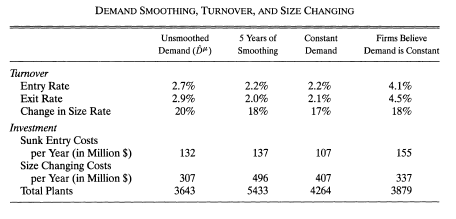
\includegraphics{cw1.png}
\end{center}
	\caption{Collard-Wexler (2013), Table VIII}
	\label{cwviii}
\end{figure}

By comparing the first two columns of results, it is evident that the smoothing policy would have mixed effects on the market.
While turnover would be reduced significantly, changes in size would not: this is consistent with the fact that, in the data, entry and exit changes seem to be uncorrelated at the market level and productivity shocks are the most likely explanation for such pattern.
Per-firm investment is unchanged by the policy -- however, more firms invest.

This increase in the number of plants in the market is probably the more notable effect of the smoothing policy: given the fixed costs to entry, peaks and troughs associated with the \textit{status-quo} large intertemporal variance of demand have asymmetric effects on the number of total plants that tend to depress market saturation.
Moreover, less such variance increases the expected profitability of a market for concave profit functions.
The conclusion is then that the \textbf{consequences of demand volatility go well beyond standard expectations of volatile investment and high turnover}; rather, demand shocks shape the structure and size distribution of the industry.




\end{document}
